\section{Faisal Najib Abdullah 1174042}
\subsection{Keterampilan Pemrograman}
\begin{enumerate}
	\item Buatlah fungsi file terpisah dengan nama NPM realtime.py untuk mendapatkan data langsung dari arduino
	\lstinputlisting[caption = Fungsi untuk mendapatkan data dari Arduino., firstline=1, lastline=7]{src/5/1174042/Praktek/1174042_realtime.py}

	\begin{figure}[H]
		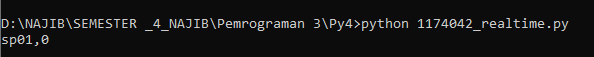
\includegraphics[width=12cm]{figures/5/1174042/Praktek/1.png}
		\centering
		\caption{Hasil dari pembacaan fungsi untuk mendapatkan data dari Arduino.}
	\end{figure}
	
	\item Buatlah fungsi file terpisah dengan nama NPM save.py untuk mendapatkan data langsung dari arduino dengan looping
	\lstinputlisting[caption = Fungsi untuk mendapatkan data langsung dari Arduino dengan looping., firstline=1, lastline=8]{src/5/1174042/Praktek/1174042_save.py}

	\begin{figure}[H]
		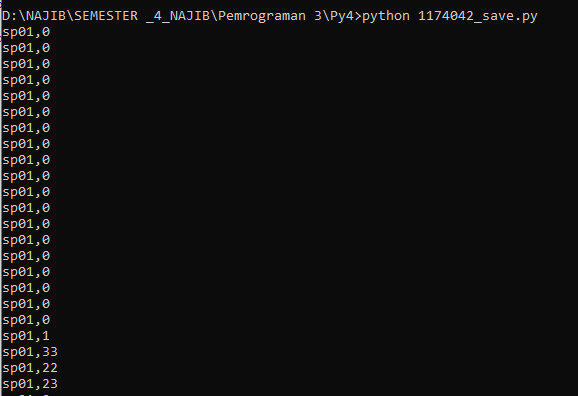
\includegraphics[width=12cm]{figures/5/1174042/Praktek/2.png}
		\centering
		\caption{Hasil dari pembacaan fungsi untuk mendapatkan data dari Arduino dengan looping.}
	\end{figure}
	
	\item Buatlah fungsi file terpisah dengan nama NPM realtime.py untuk mendapatkan data dari arduino dan langsung ditulis kedalam file csv
	\lstinputlisting[caption = Fungsi untuk mendapatkan data dari Arduino dan langsung ditulis kedalam file CSV., firstline=9, lastline=23]{src/5/1174042/Praktek/1174042_realtime.py}

	\begin{figure}[H]
		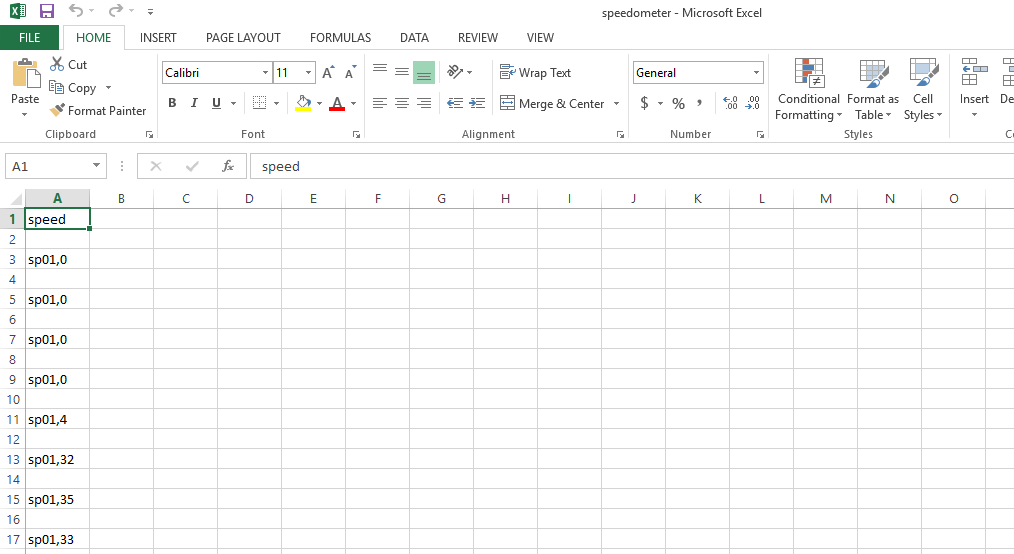
\includegraphics[width=12cm]{figures/5/1174042/Praktek/3.png}
		\centering
		\caption{Hasil dari pembacaan fungsi untuk mendapatkan data dari Arduino dan langsung ditulis kedalam file CSV.}
	\end{figure}
	
	\item Buatlah fungsi file terpisah dengan nama NPM csv.py untuk membaca file csv hasil arduino dan mengembalikan ke fungsi
	\lstinputlisting[caption = Fungsi untuk membaca file CSV hasil Arduino dan mengembalikan fungsi., firstline=1, lastline=9]{src/5/1174042/Praktek/1174042_csv.py}

	\begin{figure}[H]
		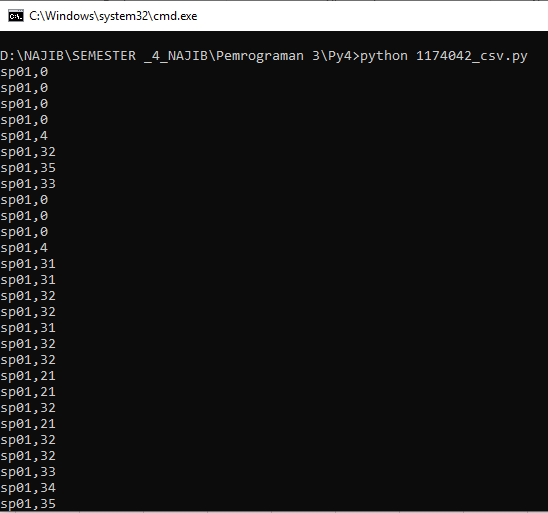
\includegraphics[width=12cm]{figures/5/1174042/Praktek/4.png}
		\centering
		\caption{Hasil dari pembacaan fungsi untuk membaca file csv hasil arduino dan mengembalikan fungsi.}
	\end{figure}
	
\end{enumerate}

\subsection{Penanganan Error}
Tuliskan  peringatan  error  yang  didapat  dari  mengerjakan  praktek  kelima  ini, dan  jelaskan  cara  penanganan  error  tersebut.   dan  Buatlah  satu  fungsi  yang menggunakan try except untuk menanggulangi error tersebut.

\hfill \break
Peringatan error di praktek kelima ini, yaitu:
\begin{itemize}
	\item Syntax Errors
	Syntax Errors adalah suatu keadaan saat kode python mengalami kesalahan penulisan. Solusinya adalah memperbaiki penulisan kode yang salah.
	
	\item Name Error
	NameError adalah exception yang terjadi saat kode melakukan eksekusi terhadap local name atau global name yang tidak terdefinisi. Solusinya adalah memastikan variabel atau function yang dipanggil ada atau tidak salah ketik.
	
	\item Type Error
	TypeError adalah exception yang akan terjadi apabila pada saat dilakukannya eksekusi terhadap suatu operasi atau fungsi dengan type object yang tidak sesuai. Solusi dari error ini adalah mengkoversi varibelnya sesuai dengan tipe data yang akan digunakan.
\end{itemize}

\hfill \break
Fungsi yang menggunakan try except untuk menanggulangi error.

\lstinputlisting[caption = Fungsi untuk menanggulangi error menggunakan Try Except., firstline=1, lastline=16]{src/5/1174042/Praktek/1174042.py}

\begin{figure}[H]
	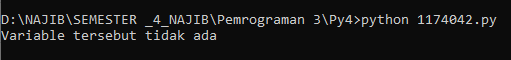
\includegraphics[width=12cm]{figures/5/1174042/Praktek/5.png}
	\centering
	\caption{Hasil pembacaan fungsi untuk menanggulangi error menggunakan Try Except.}
\end{figure}

\section{Hagan Rowlenstino/1174040}
	\subsection{Soal 1} 
		membuat fungsi untuk mendapatkan data langsung dari arduino. disini saya menggunakan arduino dengan servo. disini saya akan menginputkan data berupa angka untuk menambahkan berapa lama cervo kembali dari letak yang di tentukan ke letak awal.

	\lstinputlisting[firstline=1, lastline=13]{src/5/1174040/Praktek/chap5_1174040_realtime.py}

	\subsection{Soal 2}
	membuat fungsi untuk mendapatkan data langsung dari arduino dengan looping. disini saya menggunakan arduino dengan servo. disini saya akan menginputkan data berupa angka untuk menambahkan berapa lama cervo kembali dari letak yang di tentukan ke letak awal.

	\lstinputlisting{src/5/1174040/Praktek/chap5_1174040_save.py}

	\subsection{Soal 3}
	membuat fungsi untuk mendapatkan data langsung dari arduino lalu me write data tersebut ke dalam file csv. disini saya menggunakan arduino dengan servo. disini saya akan menginputkan data berupa angka untuk menambahkan berapa lama cervo kembali dari letak yang di tentukan ke letak awal. Nilai inputan tersebutlah yang saya  write ke dalam file 1174040\_realtime2.csv

	\lstinputlisting[firstline=15, lastline=26]{src/5/1174040/Praktek/chap5_1174040_realtime.py}

	\subsection{Soal 4}
	
	fungsi untuk membaca csv yang brisikan data dari arduino tadi :

	\lstinputlisting{src/5/1174040/Praktek/chap5_1174040_csv.py}

	\subsection{Penanganan Error}
	Disini saya mendapatkan Error yaitu FileNotFoundError dimana ada kesalahan saat menginputkan nama file yang akan digunakan, untuk penanganannya yaitu dengan cara menginputkan nama file yang benar 

	\lstinputlisting{src/5/1174040/Praktek/chap5_1174040_err.py}
	
\section{Irvan Rizkiansyah/1174043}
	\subsection{Nomor 1}
		\lstinputlisting[firstline=12, lastline=20]{src/5/1174043/Praktek/chap5_1174043_realtime.py}
		
	\subsection{Nomor 2}
		\lstinputlisting[firstline=8, lastline=22]{src/5/1174043/Praktek/chap5_1174043_simpan.py}
	
	\subsection{Nomor 3}
		\lstinputlisting[firstline=22, lastline=33]{src/5/1174043/Praktek/chap5_1174043_realtime.py}
	
	\subsection{Nomor 4}
		\lstinputlisting[firstline=8, lastline=16]{src/5/1174043/Praktek/chap5_1174043_csv.py}
		
	\subsection{Penanganan Error}
		\lstinputlisting[firstline=8, lastline=19]{src/5/1174043/Praktek/chap5_1174043_error.py}
		
\section{Luthfi Muhammad Nabil/1174035}
	\subsection{Soal 1}
	Membuat fungsi untuk mengambil data langsung dari arduino. 
	\lstinputlisting[firstline=1, lastline=5]{src/5/1174035/Praktek/chap5_1174035_realtime.py}
	\begin{figure}[H]
		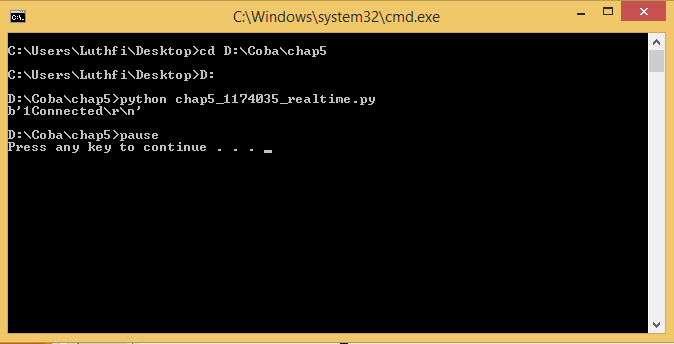
\includegraphics[width=12cm]{figures/5/1174035/Praktek/ReadNonLoop.png}
		\centering
		\caption{Hasil dari Ambil Data tanpa perulangan}
	\end{figure}
	\subsection{Soal 2}
	Membuat fungsi untuk mengambil data langsung dari arduino dengan looping. 
	\lstinputlisting{src/5/1174035/Praktek/chap5_1174035_save.py}
	\begin{figure}[H]
		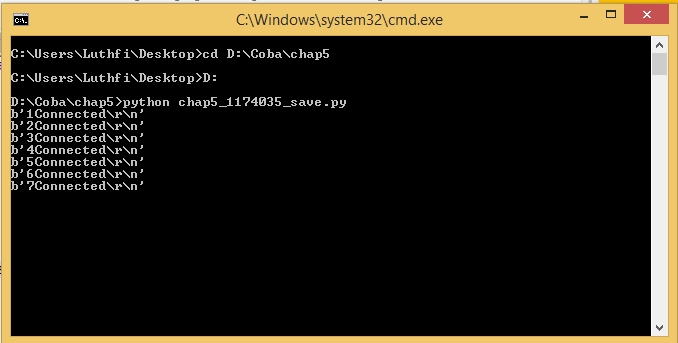
\includegraphics[width=12cm]{figures/5/1174035/Praktek/ReadLoop.png}
		\centering
		\caption{Hasil dari Ambil Data dengan perulangan}
	\end{figure}
	\subsection{Soal 3}
	Membuat fungsi untuk mengambil data langsung dari arduino lalu me write data tersebut ke dalam file csv.
	\lstinputlisting[firstline=7]{src/5/1174035/Praktek/chap5_1174035_realtime.py}
	\begin{figure}[H]
		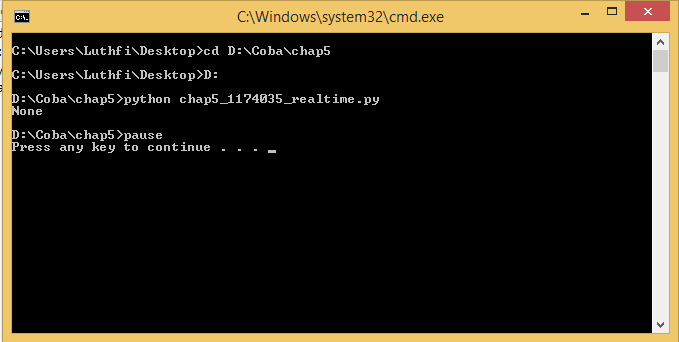
\includegraphics[width=12cm]{figures/5/1174035/Praktek/WriteCSV.png}
		\centering
		\caption{Menulis data dari serial ke file CSV}
	\end{figure}
	\begin{figure}[H]
		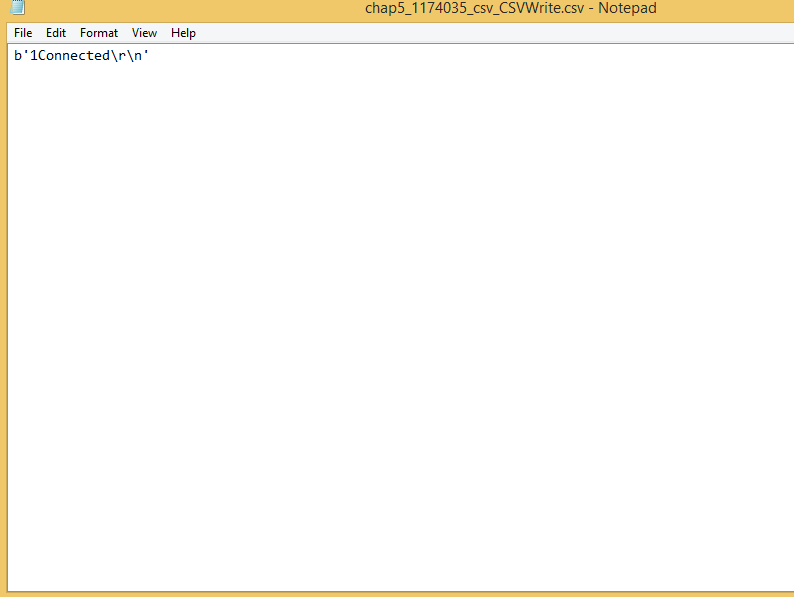
\includegraphics[width=12cm]{figures/5/1174035/Praktek/HasilCSV.png}
		\centering
		\caption{Hasil Tulis CSV dengan ambilan tanpa loop}
	\end{figure}
	\subsection{Soal 4}
	Fungsi untuk membaca csv yang berisikan data dari isi serial arduino yang dibaca sebelumnya :
	\lstinputlisting{src/5/1174035/Praktek/chap5_1174035_save.py}
	
	\subsection{Penanganan Error}
	Error yang didapat : Serial Exception
	Definisi : Serial Exception terjadi saat koneksi antara serial dan komputer terjadi masalah atau tidak dapat berkomunikasi. Untuk menangani error tersebut dapat menggunakan Try Except.
	
	Pemakaian : \lstinputlisting{src/5/1174035/Praktek/chap5_1174035_error.py}
	
	Hasil (Saat Error) dapat dilihat pada gambar \ref{Error_1174035}
	\begin{figure}[H]
		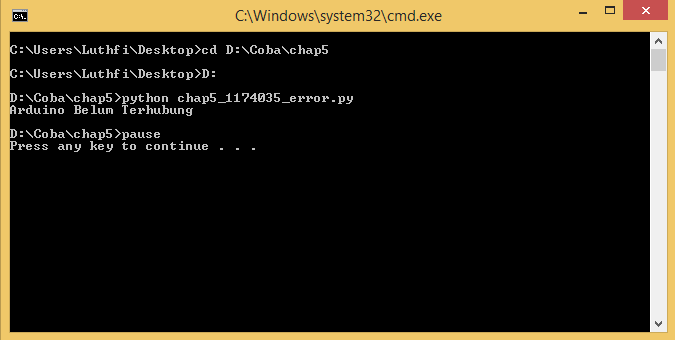
\includegraphics[width=12cm]{figures/5/1174035/Praktek/Error.png}
		\centering
		\caption{Hasil dari Error}
		\label{Error_1174035}
	\end{figure}
	
	\section{Dika Sukma Pradana 1174050}
\subsection{Keterampilan Pemrograman}
\begin{enumerate}
	\item Buatlah fungsi file terpisah dengan nama NPM realtime.py untuk mendapatkan data langsung dari arduino
	\lstinputlisting[caption = Fungsi untuk mendapatkan data dari Arduino., firstline=1, lastline=7]{src/5/1174050/Praktek/1174050_realtime.py}

	\begin{figure}[H]
		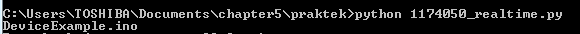
\includegraphics[width=12cm]{figures/5/1174050/Praktek/realtime.png}
		\centering
		\caption{Hasil dari pembacaan fungsi untuk mendapatkan data dari Arduino.}
	\end{figure}
	
	\item Buatlah fungsi file terpisah dengan nama NPM save.py untuk mendapatkan data langsung dari arduino dengan looping
	\lstinputlisting[caption = Fungsi untuk mendapatkan data langsung dari Arduino dengan looping., firstline=1, lastline=8]{src/5/1174050/Praktek/1174050_save.py}

	\begin{figure}[H]
		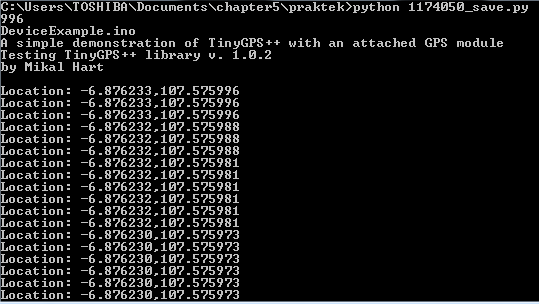
\includegraphics[width=12cm]{figures/5/1174050/Praktek/save.png}
		\centering
		\caption{Hasil dari pembacaan fungsi untuk mendapatkan data dari Arduino dengan looping.}
	\end{figure}
	
	\item Buatlah fungsi file terpisah dengan nama NPM realtime.py untuk mendapatkan data dari arduino dan langsung ditulis kedalam file csv
	\lstinputlisting[caption = Fungsi untuk mendapatkan data dari Arduino dan langsung ditulis kedalam file CSV., firstline=9, lastline=23]{src/5/1174050/Praktek/1174050_realtime.py}

	\begin{figure}[H]
		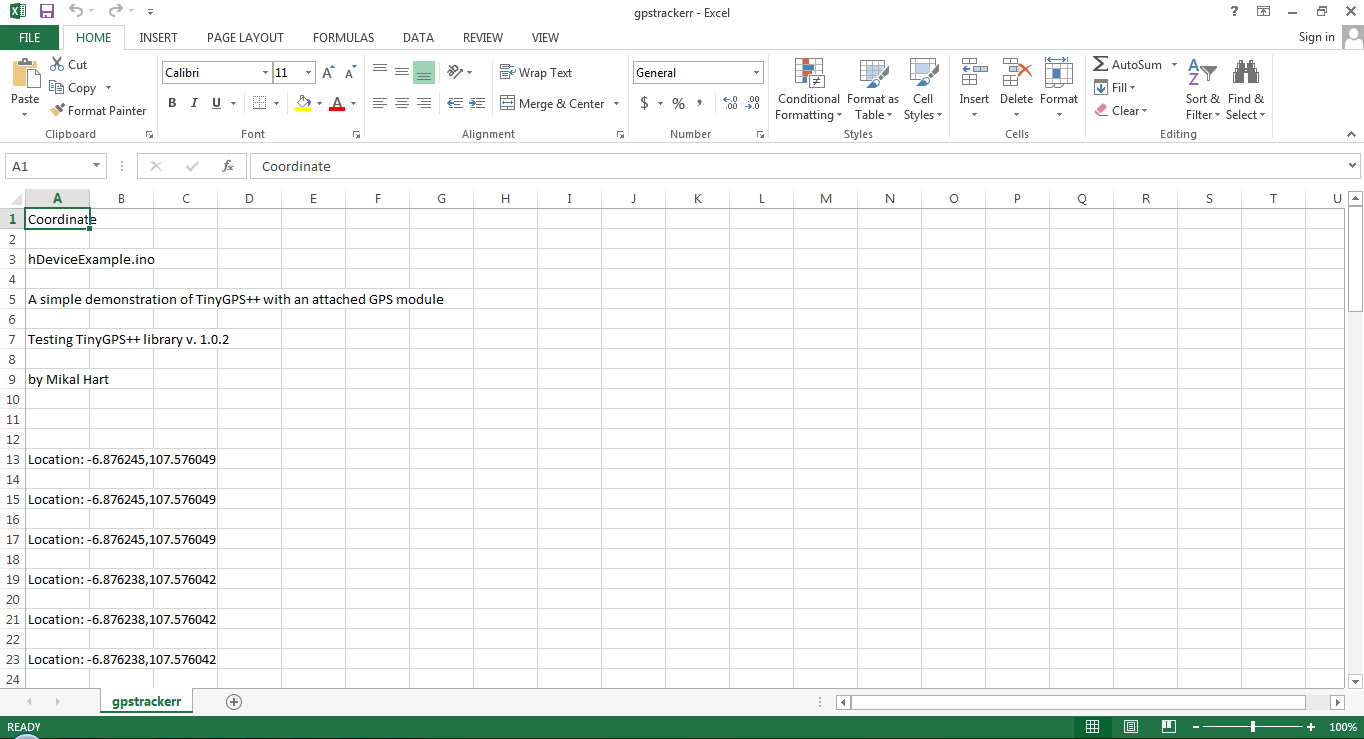
\includegraphics[width=12cm]{figures/5/1174050/Praktek/csvfile.png}
		\centering
		\caption{Hasil dari pembacaan fungsi untuk mendapatkan data dari Arduino dan langsung ditulis kedalam file CSV.}
	\end{figure}
	
	\item Buatlah fungsi file terpisah dengan nama NPM csv.py untuk membaca file csv hasil arduino dan mengembalikan ke fungsi
	\lstinputlisting[caption = Fungsi untuk membaca file CSV hasil Arduino dan mengembalikan fungsi., firstline=1, lastline=9]{src/5/1174050/Praktek/1174050_csv.py}

	\begin{figure}[H]
		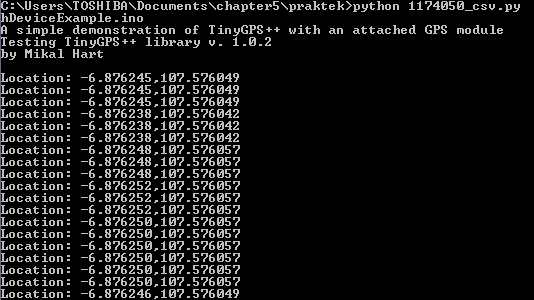
\includegraphics[width=12cm]{figures/5/1174050/Praktek/csvv.png}
		\centering
		\caption{Hasil dari pembacaan fungsi untuk membaca file csv hasil arduino dan mengembalikan fungsi.}
	\end{figure}
	
\end{enumerate}

\subsection{Penanganan Error}
Tuliskan  peringatan  error  yang  didapat  dari  mengerjakan  praktek  kelima  ini, dan  jelaskan  cara  penanganan  error  tersebut.   dan  Buatlah  satu  fungsi  yang menggunakan try except untuk menanggulangi error tersebut.

\hfill \break
Peringatan error di praktek kelima ini, yaitu:
\begin{itemize}
	\item Syntax Errors
	Syntax Errors adalah suatu keadaan saat kode python mengalami kesalahan penulisan. Solusinya adalah memperbaiki penulisan kode yang salah.
	
	\item Name Error
	NameError adalah exception yang terjadi saat kode melakukan eksekusi terhadap local name atau global name yang tidak terdefinisi. Solusinya adalah memastikan variabel atau function yang dipanggil ada atau tidak salah ketik.
	
	\item Type Error
	TypeError adalah exception yang akan terjadi apabila pada saat dilakukannya eksekusi terhadap suatu operasi atau fungsi dengan type object yang tidak sesuai. Solusi dari error ini adalah mengkoversi varibelnya sesuai dengan tipe data yang akan digunakan.
\end{itemize}

\hfill \break
Fungsi yang menggunakan try except untuk menanggulangi error.

\lstinputlisting[caption = Fungsi untuk menanggulangi error menggunakan Try Except., firstline=1, lastline=16]{src/5/1174050/Praktek/1174050.py}

\begin{figure}[H]
	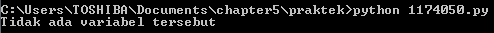
\includegraphics[width=12cm]{figures/5/1174050/Praktek/error.png}
	\centering
	\caption{Hasil pembacaan fungsi untuk menanggulangi error menggunakan Try Except.}
\end{figure}
	